\chapter{Image Stitching and Mosaicking}
\label{ch:lesson25}

This chapter brings together feature detection and matching (Chapter~\ref{ch:lesson20}), robust fitting (Chapter~\ref{ch:lesson23}), and homography estimation (Chapter~\ref{ch:lesson24}) into a complete pipeline that stitches two overlapping photos into a single seamless panorama.

\section{The pipeline, at a glance}

\begin{enumerate}
  \item \textbf{Detect and match features} between the two photos (Chapter~\ref{ch:lesson20}: SIFT $+$ ratio test).
  \item \textbf{Estimate a homography} relating one image's plane to the other's, robustly (Chapter~\ref{ch:lesson24}'s homography, Chapter~\ref{ch:lesson23}'s RANSAC).
  \item \textbf{Warp} one image into the other's coordinate frame (Chapter~\ref{ch:lesson09}: \code{cv2.warpPerspective}).
  \item \textbf{Composite and blend} the two images onto one canvas, feathering across the overlap so the seam is invisible.
\end{enumerate}

\section{An example}

\subsection*{Two overlapping photos}

Two photos of the same brick building (Figure~\ref{fig:l25-1}), taken from slightly different positions with substantial overlap.

\begin{figure}[h]
\centering
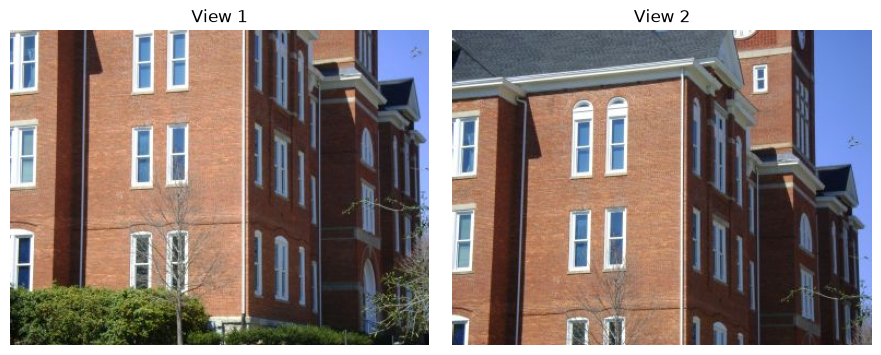
\includegraphics[width=0.9\textwidth]{figures/lesson25_fig01.png}
\caption{The two input views. \attrib{Photo: Stan Birchfield.}}
\label{fig:l25-1}
\end{figure}

\subsection*{Step 1: feature matching}

SIFT finds $938$ keypoints in view 1 and $708$ in view 2; Lowe's ratio test keeps $315$ good matches, shown in Figure~\ref{fig:l25-2}.

\begin{figure}[h]
\centering
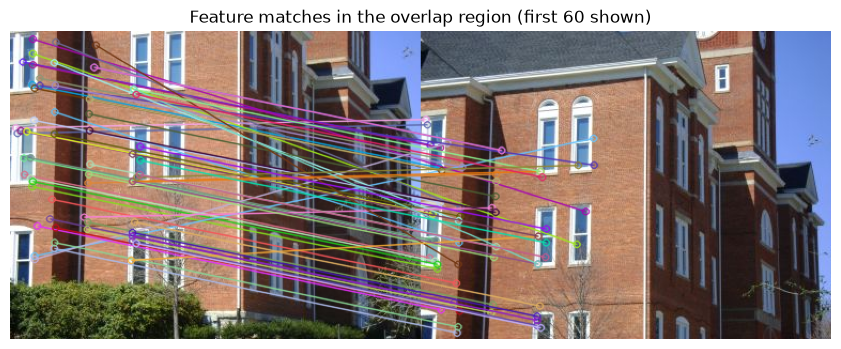
\includegraphics[width=0.9\textwidth]{figures/lesson25_fig02.png}
\caption{Feature matches in the overlap region (first 60 shown).}
\label{fig:l25-2}
\end{figure}

\subsection*{Step 2: robust homography}

Solve for the homography that maps points in view 2 into view 1's coordinate frame, so warping view 2 through it lands it in the right place on a shared canvas: \code{cv2.findHomography} with RANSAC finds $263$ of $315$ matches as inliers.

\subsection*{Steps 3-4: warp, composite, and blend}

First, figure out how big the output canvas needs to be, by mapping both images' corners through $H$ (Chapter~\ref{ch:lesson24}) and taking the bounding box --- unlike a synthetic case, these photos aren't simple axis-aligned crops of a shared frame, so the canvas size and the offset of view 1 within it both have to be computed rather than assumed. Warp view 2 onto that canvas, then blend the overlap region with a simple \textbf{feather}: a linear alpha ramp from ``fully view 1'' to ``fully view 2'' across the overlap, the same weighted-sum blending as \code{cv2.addWeighted} in Chapter~\ref{ch:lesson02}, just with a spatially-varying weight instead of a constant one. Figure~\ref{fig:l25-3} shows the resulting panorama.

\begin{figure}[h]
\centering
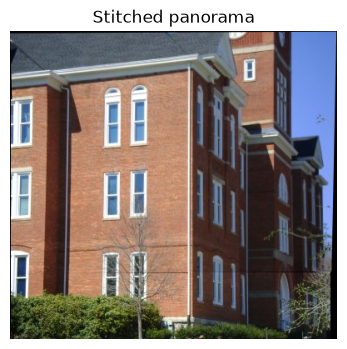
\includegraphics[width=0.6\textwidth]{figures/lesson25_fig03.png}
\caption{The stitched panorama. The roof (top, fully visible only in view 2) and the bush (bottom, fully visible only in view 1) both appear in the mosaic, confirming that the composite genuinely draws from both source images.}
\label{fig:l25-3}
\end{figure}

\subsection*{How good is the fit?}

There's no synthetic ground truth to compare against with a real photograph, but we don't need one: the RANSAC inliers themselves give a direct measure of geometric fit. For each inlier correspondence, project the point from view 2 through $H$ and measure the distance to its matched point in view 1 --- the \textbf{reprojection error}. Here: mean reprojection error $0.520$ px, max $2.919$ px --- sub-pixel-scale error, well under the RANSAC inlier threshold of 3 px, confirming $H$ is a good geometric fit, consistent with the clean seam visible in the stitched panorama. Figure~\ref{fig:l25-4} histograms the reprojection error across all inliers.

\begin{figure}[h]
\centering
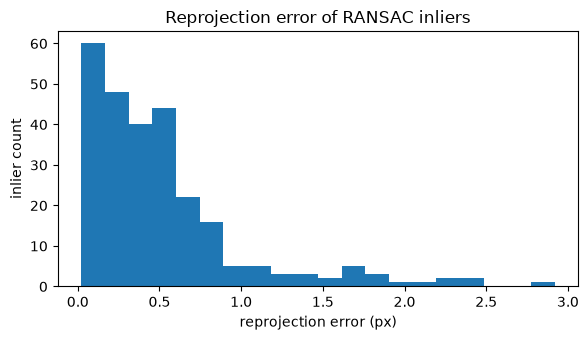
\includegraphics[width=0.55\textwidth]{figures/lesson25_fig04.png}
\caption{Reprojection error of the RANSAC inliers, histogrammed.}
\label{fig:l25-4}
\end{figure}

\section{In practice: \code{cv2.Stitcher}}

OpenCV bundles this entire pipeline (plus more robust blending, exposure compensation, and support for many images at once) behind a single high-level call. Its default \code{PANORAMA} mode assumes the images come from a camera rotating about its optical center, and warps each image onto a sphere before compositing --- great for wide panoramas, but it bows straight lines when the scene is dominated by flat, rectilinear structure (like a building facade) and the camera translated rather than purely rotated. \code{SCANS} mode instead composites with the planar homographies directly, matching the approach used above, as confirmed by the successful \code{Stitcher} run in Figure~\ref{fig:l25-5}.

\begin{figure}[h]
\centering
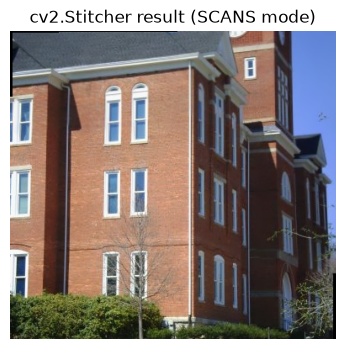
\includegraphics[width=0.5\textwidth]{figures/lesson25_fig05.png}
\caption{\code{cv2.Stitcher} in \code{SCANS} mode: status \code{OK}.}
\label{fig:l25-5}
\end{figure}

\subsection*{Exercises}
\begin{enumerate}
  \item Reduce the overlap between the two views (e.g.\ crop view 2 down to its rightmost quarter before matching). At what point does SIFT matching find too few good matches for \code{findHomography} to produce a reliable result?
  \item Replace the linear feather with a hard cutoff (no blending: just pick whichever image covers each pixel, splitting the overlap down the middle) and compare the visible seam quality to the feathered version.
  \item $H$ here is a mild general homography, not a pure translation, because the two photos were taken from slightly different positions rather than a pure sideways pan. Print the ratio of $H$'s last row to $[0,0,1]$ as a rough measure of how much perspective distortion it captures, and compare it to what you'd get by forcing an affine fit (\code{cv2.estimateAffinePartial2D}) instead --- how well does the affine approximation stitch the images compared to the full homography?
\end{enumerate}

\vfill
\fullcode{lesson25}{lesson25_stitching_mosaicking}
